\documentclass{standalone}
\usepackage{tikz}
\usetikzlibrary{shapes.geometric}
\begin{document}
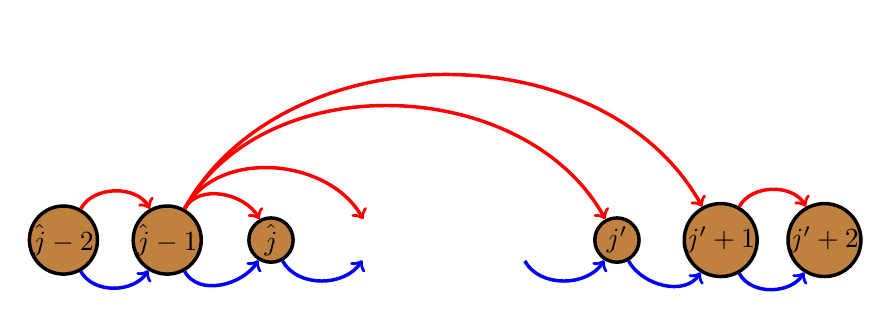
\begin{tikzpicture}
[every node/.style={inner sep=0pt}]
\node (1) [circle, minimum size=16.0pt, fill=brown, line width=1.25pt, draw=black] at (25.0pt, -62.5pt) {\textcolor{black}{$\hat{j}-2$}};
\node (2) [circle, minimum size=16.0pt, fill=brown, line width=1.25pt, draw=black] at (62.5pt, -62.5pt) {\textcolor{black}{$\hat{j}-1$}};
\node (3) [circle, minimum size=16.0pt, fill=brown, line width=1.25pt, draw=black] at (100.0pt, -62.5pt) {\textcolor{black}{$\hat{j}$}};
\node (7) [circle, minimum size=16.0pt, fill=white, line width=1.25pt] at (137.5pt, -62.5pt)  {};
\ldots
\node (4) [circle, minimum size=16.0pt, fill=brown, line width=1.25pt, draw=black] at (225.0pt, -62.5pt) {\textcolor{black}{$j'$}};
\node (8) [circle, minimum size=16.0pt, fill=white, line width=1.25pt] at (187.5pt, -62.5pt)  {};
\node (5) [circle, minimum size=16.0pt, fill=brown, line width=1.25pt, draw=black] at (262.5pt, -62.5pt) {\textcolor{black}{$j'+1$}};
\node (6) [circle, minimum size=16.0pt, fill=brown, line width=1.25pt, draw=black] at (300.0pt, -62.5pt) {\textcolor{black}{$j'+2$}};
\draw [line width=1.25, ->, color=blue] (1) to  [in=238, out=299] (2);
\draw [line width=1.25, ->, color=blue] (2) to  [in=238, out=299] (3);
\draw [line width=1.25, ->, color=blue] (3) to  [in=238, out=299] (7);
\draw [line width=1.25, ->, color=blue] (8) to  [in=238, out=299] (4);
\draw [line width=1.25, ->, color=blue] (4) to  [in=238, out=299] (5);
\draw [line width=1.25, ->, color=blue] (5) to  [in=238, out=299] (6);
\draw [line width=1.25, ->, color=red] (1) to  [in=119, out=61] (2);
\draw [line width=1.25, ->, color=red] (2) to  [in=119, out=61] (3);
\draw [line width=1.25, ->, color=red] (2) to  [in=119, out=61] (7);
\draw [line width=1.25, ->, color=red] (2) to  [in=119, out=61] (4);
\draw [line width=1.25, ->, color=red] (2) to  [in=119, out=61] (5);
\draw [line width=1.25, ->, color=red] (5) to  [in=119, out=61] (6);
\end{tikzpicture}
\end{document}
